%-*- coding: UTF-8 -*-
% gougu.tex
% 勾股定理
\documentclass[hyperref,UTF8,c5size]{ctexart} 
% ctexart, ctexrep, ctexbook 分别用来写中文短文,中文报告,中文书籍 
% ctexart默认时标题不独自成页的,可加入选项titlepage修改为独自成页
% c5size表示正文正五号字体
% 2.4.1

\usepackage[colorlinks,linkcolor=black,bookmarksnumbered=true,backref=true,bookmarks=true,bookmarksopen=true]{hyperref}  
% hyperref超连接、书签
% 3.2.3

% \usepackage[raggedright]{titlesec}
% titlesec宏包可用来全局的改变标题的字体、字号、对齐方式
% raggedright将标题左对齐(效果是这样的)
% usepackage可能与CTEXsetup设置标题冲突,可能重复输出序号如二2
% 2.3.4
\usepackage{graphicx}
% 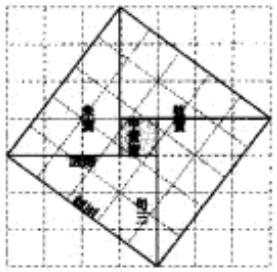
\includegraphics[scale=0.6]{xiantu.png}
\usepackage{float}
% \begin{table}[H] 
\usepackage{amsmath}
% 满足式\eqref{eq:gougu}的整数称为\emph{勾股数}。
\usepackage{geometry}
\geometry{a4paper,centering,scale=0.8}
% 设计页面尺寸
% 2.4.2
\usepackage[format=hang,font=small,textfont=it]{caption}
% 改变图标标题格式
% \usepackage[nottoc]{tocbibind} 
% tocbibind默认把章节目录、图标目录、文献、索引加入章节目录里
% 选项可进行进一步控制,nottoc不加入章节目录(默认目录自己会出现在目录里)
% 3.1.2
\newenvironment{myquote}
{\begin{quote}\kaishu\zihao{-5}}
{\end{quote}}
% 定义新环境
\newcommand\degree{^\circ} 
% 定义新命令
% ^表示上标,\circ表示函数复合的二元运算符。
% _表示下标
% 数学符号4.3

\newtheorem{thm}{定理}
% 定理类环境
% 2.2.4


\title{\heiti\zihao{2}数据库系统实验\\实验报告}
\author{\kaishu 吴育滨\\王\hspace{1em}五}
\date{}
% title author date 可以放在maketitle前的任何位置,通常放在导言区 date可以省略,默认为今天
% 字号0为出好,-0为小初号,1为一号,-1为小一号
% em为字号对应的长度
% 2.1.4

% \bibliographystyle{plain}
% \bibliographystyle命令设定参考文献格式,通常在导言区完成。
% 基本的Bibtex文献格式包括plain、unsrt、alpha和abbrv
% plain格式按作者、日期标题排序
% 文档中使用\cite引用文献
% 文档中用\nocite命令指明不引用但仍列出文献标签
% \bibliography{math}指明文献库
% 引用bib文献,需
% a、先xelatex *.tex源文件编译,将\cite,\bibliography,\bibliographystyle写入.aux辅助文件,生成无文献PDF
% b、然后运行bibtex *.aux生成.bbl文献列表
% c、xelatex *.tex,依靠*.aux *.bbl生成有文献无引用PDF,同时将\cite应用信息写入.aux
% d、xelatex *.tex,依靠*.aux *.bbl,在应用处生存引用信息,得到最终PDF
% 可使用JabRef生存.bib
% 3.3.1

\usepackage{tabularx}
% 定长表格
% 5.1.3

\usepackage{listings}
\usepackage{xcolor}
\lstset{
    frame=shadowbox,
    rulesepcolor=\color{red!20!green!20!blue!20}
}
% 程序代码块
% 2.2.5.2
\CTEXsetup[number={\chinese{section}},format={\raggedright}, nameformat={\LARGE\bfseries}, titleformat={\LARGE\bfseries}]{section}
% \CTEXsetup[name={第,章}, aftername={---} ,format={\raggedright}, nameformat={\Large\bfseries}, titleformat={\LARGE\sffamily}, indent={1pc}]{chapter}
% 2.3.4

\usepackage{tocloft}
\renewcommand\cfttoctitlefont{\LARGE\bfseries}
% \CTEXsetup改变section的的format为左对其后,\contentsname的也左对齐了,且格式消失了
% 使用tocloft修改\contentsname字体格式
% 3.1.3

%这里之前称为导言区preamble,这里正式开始文档
\begin{document}
    %\vspace*{\fill}
    \begin{center}
    \normalfont
    {\Huge\bfseries 数据库系统实验\\实验报告}

    \bigskip
    \begin{table}[H]
            \centering
            %\label{tab:diff_quotient}
            \begin{tabularx}{0.8\textwidth}{|@{\hspace{1em}}c@{\hspace{1em}}@{\extracolsep{1em}}*{1}{|X}|}
            \hline
            {\bfseries 题目} & {\bfseries (实验3)}\\
            \hline 
            {\bfseries 姓名} & 吴育滨\\
            \hline
            {\bfseries 学号} & 13349126\\
            \hline
            {\bfseries 班级} & 计科2班\\
            \hline
            \end{tabularx}
    \end{table}
    % 使用了宏包tabularx
    % 5.1.3
    %{\Large\itshape 吴育滨}

    %\medskip
    %\today

    \end{center}
    %\vspace*{\stretch{3}}

% \maketitle
% \maketitle通常为document的第一个指令,前面的ctexart默认不单独成页,ctexrep、ctexbook默认单独成页
% 可通过文档类选项notitlepage修改不单独成页
% title可不通过\title \maketitle命令得到,直接手工排版得到,
% 2.3.1
% 不单独成页的\maketitle、单独成页的\part以及\chapter命令所在的一页,使用plain风格只显示页码
% 2.4.3

% \thispagestyle{empty}
% maketitle默认此页的页面格式为plain
% \thispagestyle{headings}单独设置此页风格
% 2.4.3

% \clearpage
% 另起新页
% 2.3.2

% \pagenumbering{roman}
% 修改页码的编号方式,此命令会使页码从1开始
% 2.4.3

% \pagestyle{plain}
% 整体设置页面风格
% 2.4.3

% \tableofcontents
% 读入.toc目录文件如果存在的话
% ctexart为section subsection subsubsection 三级目录
% ctexrep、ctexbook为chapter section subsection 三级目录
% 可以通过修改计数器tocdepth来控制目录的深度 
% 3.1.1
% 3.1.2

% \clearpage
% \pagenumbering{arabic}
% \pagestyle{headings}

\pagestyle{plain}
\section{实验环境}
% ctexart的最高层
% ctexrep、ctexbook的最高层为chapter
% 三种文档类还有一个可选的最高层part
% \appendix为附录开始,改用字母标号
% 2.3.2 表2.13 章节层次
        \begin{tabular}{@{}l@{:}l}
        1、{\bfseries 操作系统} & ubuntu 14.04 LTS; \\
        2、{\bfseries DBMS}  & mysql 5.5.44; \\
        3、{\bfseries 图形界面} & mysql-workbench 6.0.8(用以生成ER图)。 \\
        \end{tabular}

\section{实验内容}
        \subsection{创建数据库以及表}
            \subsubsection{创建报纸编码表(paper)}
                paper代码,建表、插入数据、查询表数据:
		            \begin{lstlisting}[language=SQL]
CREATE TABLE `paper` (
  `pno` char(6) NOT NULL DEFAULT '',
  `pna` varchar(20) DEFAULT NULL,
  `ppr` decimal(4,2) DEFAULT NULL,
  PRIMARY KEY (`pno`)
) ENGINE=InnoDB DEFAULT CHARSET=utf8;
INSERT INTO `paper` VALUES 
('000001','人民日报',12.50),
('000002','解放军报',14.50),
('000003','光明日报',10.50),
('000004','青年报',11.50),
('000005','扬子日报',18.50);
select * from `paper`;
                    \end{lstlisting}

                    运行结果:
		            \begin{lstlisting}
+--------+--------------+-------+
| pno    | pna          | ppr   |
+--------+--------------+-------+
| 000001 | 人民日报     | 12.50 |
| 000002 | 解放军报     | 14.50 |
| 000003 | 光明日报     | 10.50 |
| 000004 | 青年报       | 11.50 |
| 000005 | 扬子日报     | 18.50 |
+--------+--------------+-------+
                    \end{lstlisting}

            \subsubsection{创建顾客编码表(customer)}
                customer代码,建表、插入数据、查询表数据:
			        \begin{lstlisting}[language=SQL]
CREATE TABLE `customer` (
  `cno` char(4) NOT NULL DEFAULT '',
  `cna` varchar(20) DEFAULT NULL,
  `adr` varchar(80) DEFAULT NULL,
  PRIMARY KEY (`cno`)
) ENGINE=InnoDB DEFAULT CHARSET=utf8;
INSERT INTO `customer` VALUES 
('0001','李涛','无锡市解放东路123号'),
('0002','钱金浩','无锡市人民西路234号'),
('0003','邓杰','无锡市惠河路432号'),
('0004','朱海红','无锡市中山东路432号'),
('0005','欧阳阳文','无锡市中山东路532号');
select * from `customer`;
			        \end{lstlisting}

                    运行结果:
		            \begin{lstlisting}
+------+--------------+-----------------------------+
| cno  | cna          | adr                         |
+------+--------------+-----------------------------+
| 0001 | 李涛         | 无锡市解放东路123号         |
| 0002 | 钱金浩       | 无锡市人民西路234号         |
| 0003 | 邓杰         | 无锡市惠河路432号           |
| 0004 | 朱海红       | 无锡市中山东路432号         |
| 0005 | 欧阳阳文     | 无锡市中山东路532号         |
+------+--------------+-----------------------------+
		            \end{lstlisting}

            \subsubsection{创建顾客订阅表(cp)}
                cp代码,建表、插入数据、查询表数据:
			        \begin{lstlisting}[language=SQL]
CREATE TABLE `cp` ( 
  `cno` char(4) NOT NULL DEFAULT '',
  `pno` char(6) NOT NULL DEFAULT '',
  `num` tinyint(4) DEFAULT NULL,
  PRIMARY KEY (`cno`,`pno`),
  KEY `pno` (`pno`),
  CONSTRAINT `cp_ibfk_1` FOREIGN KEY (`cno`) REFERENCES `customer` (`cno`),
  CONSTRAINT `cp_ibfk_2` FOREIGN KEY (`pno`) REFERENCES `paper` (`pno`) 
) ENGINE=InnoDB DEFAULT CHARSET=utf8;
INSERT INTO `cp` VALUES 
('0001','000001',2),
('0001','000002',4),
('0001','000005',6),
('0002','000001',2),
('0002','000003',2),
('0002','000005',2),
('0003','000003',2),
('0003','000004',4),
('0004','000001',1),
('0004','000003',3),
('0004','000005',2),
('0005','000001',4),
('0005','000002',1),
('0005','000003',4),
('0005','000004',3),
('0005','000005',5);
select * from `cp`;
			        \end{lstlisting}

                    运行结果:
                    \begin{lstlisting}
+------+--------+------+
| cno  | pno    | num  |
+------+--------+------+
| 0001 | 000001 |    2 |
| 0001 | 000002 |    4 |
| 0001 | 000005 |    6 |
| 0002 | 000001 |    2 |
| 0002 | 000003 |    2 |
| 0002 | 000005 |    2 |
| 0003 | 000003 |    2 |
| 0003 | 000004 |    4 |
| 0004 | 000001 |    1 |
| 0004 | 000003 |    3 |
| 0004 | 000005 |    2 |
| 0005 | 000001 |    4 |
| 0005 | 000002 |    1 |
| 0005 | 000003 |    4 |
| 0005 | 000004 |    3 |
| 0005 | 000005 |    5 |
+------+--------+------+
                    \end{lstlisting}

    \subsection{创建和使用视图}
        \subsubsection{创建视图C\_P\_N}
            C\_P\_N代码,建视图、查询视图数据:
		    \begin{lstlisting}[language=SQL]
CREATE VIEW `C_P_N` AS 
select `customer`.`cno`,`customer`.`cna`,`pno`,`pna`,`num`
from `customer` natural join `cp` natural join `paper`;
select * from `C_P_N`;
		    \end{lstlisting}

            运行结果:
            \begin{lstlisting}
+------+--------------+--------+--------------+------+
| cno  | cna          | pno    | pna          | num  |
+------+--------------+--------+--------------+------+
| 0001 | 李涛         | 000001 | 人民日报     |    2 |
| 0002 | 钱金浩       | 000001 | 人民日报     |    2 |
| 0004 | 朱海红       | 000001 | 人民日报     |    1 |
| 0005 | 欧阳阳文     | 000001 | 人民日报     |    4 |
| 0001 | 李涛         | 000002 | 解放军报     |    4 |
| 0005 | 欧阳阳文     | 000002 | 解放军报     |    1 |
| 0002 | 钱金浩       | 000003 | 光明日报     |    2 |
| 0003 | 邓杰         | 000003 | 光明日报     |    2 |
| 0004 | 朱海红       | 000003 | 光明日报     |    3 |
| 0005 | 欧阳阳文     | 000003 | 光明日报     |    4 |
| 0003 | 邓杰         | 000004 | 青年报       |    4 |
| 0005 | 欧阳阳文     | 000004 | 青年报       |    3 |
| 0001 | 李涛         | 000005 | 扬子日报     |    6 |
| 0002 | 钱金浩       | 000005 | 扬子日报     |    2 |
| 0004 | 朱海红       | 000005 | 扬子日报     |    2 |
| 0005 | 欧阳阳文     | 000005 | 扬子日报     |    5 |
+------+--------------+--------+--------------+------+
            \end{lstlisting}
        
        \subsubsection{修改视图C\_P\_N}
            C\_P\_N代码,修改视图、查询视图数据:
		    \begin{lstlisting}[language=SQL]
ALTER VIEW `C_P_N` AS 
select `customer`.`cno`,`customer`.`cna`,`pno`,`pna`,`num`,`ppr`
from `customer` natural join `cp` natural join `paper`;
select * from `C_P_N`;
		    \end{lstlisting}

            运行结果:
            \begin{lstlisting}
+------+--------------+--------+--------------+------+-------+
| cno  | cna          | pno    | pna          | num  | ppr   |
+------+--------------+--------+--------------+------+-------+
| 0001 | 李涛         | 000001 | 人民日报     |    2 | 12.50 |
| 0002 | 钱金浩       | 000001 | 人民日报     |    2 | 12.50 |
| 0004 | 朱海红       | 000001 | 人民日报     |    1 | 12.50 |
| 0005 | 欧阳阳文     | 000001 | 人民日报     |    4 | 12.50 |
| 0001 | 李涛         | 000002 | 解放军报     |    4 | 14.50 |
| 0005 | 欧阳阳文     | 000002 | 解放军报     |    1 | 14.50 |
| 0002 | 钱金浩       | 000003 | 光明日报     |    2 | 10.50 |
| 0003 | 邓杰         | 000003 | 光明日报     |    2 | 10.50 |
| 0004 | 朱海红       | 000003 | 光明日报     |    3 | 10.50 |
| 0005 | 欧阳阳文     | 000003 | 光明日报     |    4 | 10.50 |
| 0003 | 邓杰         | 000004 | 青年报       |    4 | 11.50 |
| 0005 | 欧阳阳文     | 000004 | 青年报       |    3 | 11.50 |
| 0001 | 李涛         | 000005 | 扬子日报     |    6 | 18.50 |
| 0002 | 钱金浩       | 000005 | 扬子日报     |    2 | 18.50 |
| 0004 | 朱海红       | 000005 | 扬子日报     |    2 | 18.50 |
| 0005 | 欧阳阳文     | 000005 | 扬子日报     |    5 | 18.50 |
+------+--------------+--------+--------------+------+-------+
            \end{lstlisting}
        
        \subsubsection{通过视图C\_P\_N实现对数据的更新操作}
            由于视图中的行和基表中的行之间具有一对一的关系,所以能通过视图C\_P\_N对数据进行更新。
		    \begin{lstlisting}[language=SQL]
update `C_P_N`
set num = num + 1
where cno = '0001';
select * from `C_P_N`;
		    \end{lstlisting}

            运行结果(可与前面视图运行结果数据对比):
            \begin{lstlisting}
+------+--------------+--------+--------------+------+-------+
| cno  | cna          | pno    | pna          | num  | ppr   |
+------+--------------+--------+--------------+------+-------+
| 0001 | 李涛         | 000001 | 人民日报     |    3 | 12.50 |
| 0002 | 钱金浩       | 000001 | 人民日报     |    2 | 12.50 |
| 0004 | 朱海红       | 000001 | 人民日报     |    1 | 12.50 |
| 0005 | 欧阳阳文     | 000001 | 人民日报     |    4 | 12.50 |
| 0001 | 李涛         | 000002 | 解放军报     |    5 | 14.50 |
| 0005 | 欧阳阳文     | 000002 | 解放军报     |    1 | 14.50 |
| 0002 | 钱金浩       | 000003 | 光明日报     |    2 | 10.50 |
| 0003 | 邓杰         | 000003 | 光明日报     |    2 | 10.50 |
| 0004 | 朱海红       | 000003 | 光明日报     |    3 | 10.50 |
| 0005 | 欧阳阳文     | 000003 | 光明日报     |    4 | 10.50 |
| 0003 | 邓杰         | 000004 | 青年报       |    4 | 11.50 |
| 0005 | 欧阳阳文     | 000004 | 青年报       |    3 | 11.50 |
| 0001 | 李涛         | 000005 | 扬子日报     |    7 | 18.50 |
| 0002 | 钱金浩       | 000005 | 扬子日报     |    2 | 18.50 |
| 0004 | 朱海红       | 000005 | 扬子日报     |    2 | 18.50 |
| 0005 | 欧阳阳文     | 000005 | 扬子日报     |    5 | 18.50 |
+------+--------------+--------+--------------+------+-------+
            \end{lstlisting}

        \subsubsection{删除视图C\_P\_N}

            代码:
            \begin{lstlisting}[language=SQL]
DROP VIEW `C_P_N`;
            \end{lstlisting}

\section{创建数据库ER图}
    customer、cp和paper三个表的数据库ER图为图\ref{fig:ER}
    \begin{figure}[H]
        \centering
        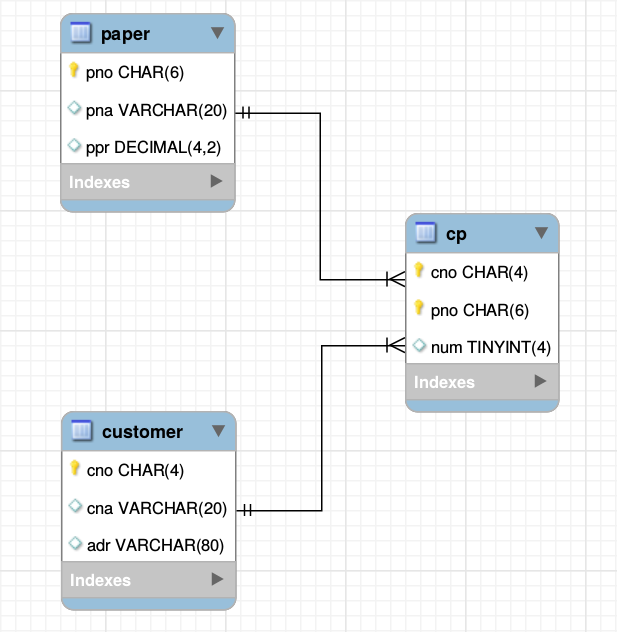
\includegraphics[scale=0.35]{db_diagram.png}
        \caption{db\_diagram(dingbao.sql的ER图)}
        \label{fig:ER}
    \end{figure}
\end{document}
